\documentclass[12pt]{article}
% Full article preamble (duplicated, no common file)
\usepackage{fontspec}
\usepackage[a4paper,margin=2.5cm,includefoot]{geometry}
\usepackage{polyglossia}
\usepackage{amsmath}
\usepackage{amssymb}
\usepackage{xcolor}
\usepackage{fancyhdr}
\usepackage{graphicx}
\usepackage{listings}
\usepackage[most]{tcolorbox}
\usepackage{pifont}
\usepackage{enumitem}
\usepackage{titlesec}
\usepackage[bottom]{footmisc}
\usepackage{titling}
\usepackage{minted}
\usepackage{etoolbox}
\usepackage{array}
\usepackage{extsizes}

\newfontfamily\emoji{Segoe UI Emoji}

\pagestyle{fancy}

\setmainlanguage[numerals=western]{arabic}
\setotherlanguage{english}
\newfontfamily\arabicfont[Script=Arabic]{Amiri}
\newfontfamily\arabicfonttt[Script=Arabic]{Courier New}

\lstset{
  language=[Sharp]C,
  numbers=left,
  stepnumber=1,
  numbersep=8pt,
  frame=single,
  basicstyle=\ttfamily\small,
  keywordstyle=\color{blue},
  stringstyle=\color{red},
  commentstyle=\color{green!50!black}
}

\newif\ifdetailed
\ifdefined\setdetailed
  \setdetailed
\fi

\newif\ifwithsols
\ifdefined\setwithsols
  \setwithsols
\fi

% unified tcolorboxes for articles
\tcbset{colback=white, colframe=black, fonttitle=\bfseries, boxrule=0.8pt}
\newtcolorbox{boxDef}[1][]{colback=blue!5!white,colframe=blue!75!black,
  title={{\emoji📘} تعريف\ifx\\#1\\\else ~#1\fi :}}
\newtcolorbox{boxExercise}[1][]{colback=cyan!5!white,colframe=cyan!70!black,
  title={{\emoji🧩} تمرين\ifx\\#1\\\else ~#1\fi :}}
\newtcolorbox{boxExample}[1][]{colback=yellow!5!white,colframe=orange!90!black,
  title={{\emoji📝} مثال\ifx\\#1\\\else ~#1\fi :}}
\newtcolorbox{boxNote}[1][]{colback=gray!10!white,colframe=black,
  title={{\emoji✨} ملاحظة\ifx\\#1\\\else ~#1\fi :}}
\newtcolorbox{boxAttention}[1][]{colback=magenta!10!white,colframe=magenta!80!black,
  title={{\emoji🔔} تنبيه\ifx\\#1\\\else ~#1\fi :}}
\newtcolorbox{boxWarning}[1][]{colback=red!5!white,colframe=red!75!black,
  title={{\emoji⚡} ملاحظة هامة\ifx\\#1\\\else ~#1\fi :}}
\newtcolorbox{boxSolution}[1][]{colback=green!5!white,colframe=green!60!black,
  title={{\emoji✅} حل\ifx\\#1\\\else ~#1\fi :}}
\newtcolorbox{boxSymbol}[1][]{colback=purple!5!white,colframe=purple!70!black,
  title={{\emoji🔣} رمز\ifx\\#1\\\else ~#1\fi :}}

\tcbset{simplecode/.style={ colback=gray!5, colframe=black!50, boxrule=0.4pt, arc=2pt, left=4pt,right=4pt,top=4pt,bottom=4pt}}
\newenvironment{boxCode}{\begin{tcolorbox}[simplecode]}{\end{tcolorbox}}

\newcolumntype{C}[1]{>{\centering\arraybackslash}p{#1}}

% redefine spaces after titles
\makeatletter
\renewcommand{\@maketitle}{%
  \begin{center}
    {\huge \bfseries \@title \par}%
    \vskip 0.2em % space between title and author
    {\large \@author \par}%
    % \vskip 0.2em % space between author and date
    % {\normalsize \@date \par}%
  \end{center}
}
\makeatother

\fancyhf{} % clear default
\fancypagestyle{plain}{
  \fancyhf{}
  \fancyhead[L]{مدرسة التسامح الشاملة}
  % \fancyhead[L]{
\includegraphics[height=1cm]{../../../images/logoTasamoh.png}}
  \fancyhead[R]{الأستاذ محمود اغبارية}
  \fancyfoot[C]{\thepage}
}

\fancyhead[L]{مدرسة التسامح الشاملة}
\fancyhead[R]{الأستاذ محمود اغبارية}
\fancyfoot[C]{\thepage}
% \date{\today}

\setcounter{tocdepth}{3} % only section subsection and subsubsection in TOC


% ----------------------


% \begin{document}

% \maketitle

% % \clearpage  % start TOC on a new page
% % \renewcommand{\contentsname}{جدول المحتويات}
% % \tableofcontents
% % \clearpage

% \part*{part 1} % the * prevents numbering
% \section*{مقدمة}
% \subsection*{مثال رياضي}
% \subsubsection*{مثال فرعي}
% \paragraph*{ paragraph 1}
% \subparagraph*{sub paragraph 1}

% \ifdetailed
% \begin{english}
% \begin{minted}{csharp}
% // C# Example
% \end{minted}
% \end{english}
% \fi

% OLD WAY
% \ifdetailed
% \begin{english}
% \begin{lstlisting}
% // C# Example
% \end{lstlisting}
% \end{english}
% \fi

% % 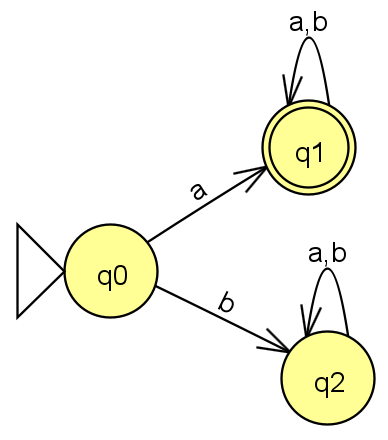
\includegraphics[width=0.2\textwidth]{../../../images/DFAs/ex1_q1.png}



% \vspace{3cm}
% \begin{flushleft}
% أرجو لكم وقتًا ممتعًا.

% الأستاذ محمود اغبارية.
% \end{flushleft}


% \end{document}


\title{وظيفة بيتية 2 للصف العاشر 10}

\begin{document}

\maketitle
\pagestyle{fancy}
\thispagestyle{fancy}

\begin{enumerate}[itemsep=1em]

    \subsection*{العمليات الحسابية الأساسية}
    \item
    ما هو مخرج الكود التالي إذا أدخل المستخدم القيمة \texttt{5}؟
    \begin{english}
        \begin{minted}{csharp}
int x = int.Parse(Console.ReadLine());
Console.WriteLine(x + 3);
        \end{minted}
    \end{english}
    \ifwithsols
    \begin{boxSolution}
        $8$
    \end{boxSolution}
    \fi

    \item
    ما هو مخرج الكود التالي إذا أدخل المستخدم \texttt{4} ثم \texttt{2}؟
    \begin{english}
        \begin{minted}{csharp}
int a = int.Parse(Console.ReadLine());
int b = int.Parse(Console.ReadLine());
Console.WriteLine(a * b);
        \end{minted}
    \end{english}
    \ifwithsols
    \begin{boxSolution}
        $8$
    \end{boxSolution}
    \fi

    \item
    ما هو مخرج الكود التالي إذا أدخل المستخدم \texttt{7} ثم \texttt{3}؟
    \begin{english}
        \begin{minted}{csharp}
int x = int.Parse(Console.ReadLine());
int y = int.Parse(Console.ReadLine());
Console.WriteLine(x / y);
        \end{minted}
    \end{english}
    \ifwithsols
    \begin{boxSolution}
        $2$ \\ انتبه أنّ النتيجة ستكون من نوع \texttt{int} وليس \texttt{double} لأنّ كل المتغيرات هي من نوع \texttt{int}.
    \end{boxSolution}
    \fi

    \ifwithsols
    \clearpage
    \fi

    \item
    ما هو مخرج الكود التالي إذا أدخل المستخدم \texttt{2.5} ثم \texttt{4}؟
    \begin{english}
        \begin{minted}{csharp}
double x = double.Parse(Console.ReadLine());
int y = int.Parse(Console.ReadLine());
Console.WriteLine(x + y);
        \end{minted}
    \end{english}
    \ifwithsols
    \begin{boxSolution}
        $9.2$
    \end{boxSolution}
    \fi

    \item
    ما هو مخرج الكود التالي إذا أدخل المستخدم:
    \begin{enumerate}[label=\Roman*.]
        \item \texttt{8} ثم \texttt{3} ؟
        \item \texttt{3} ثم \texttt{8} ؟
        \item \texttt{3} ثم \texttt{9} ؟
        \item \texttt{21} ثم \texttt{6} ؟
    \end{enumerate}
    \begin{english}
        \begin{minted}{csharp}
int a = int.Parse(Console.ReadLine());
int b = int.Parse(Console.ReadLine());
Console.WriteLine(a % b);
        \end{minted}
    \end{english}
    \ifwithsols
    \begin{boxSolution}
        \begin{enumerate}[label=\Roman*.]
        \item $2$
        \item $3$
        \item $0$
        \item $3$
    \end{enumerate}
    \end{boxSolution}
    \fi

%%%%%%%%%%%%%%%%%%%%%%%%%%%%%%%%%%%%%%%%%%%%%%
    \clearpage
    \subsection*{ترتيب العمليات الحسابية}

    \item
    ما هو مخرج الكود التالي؟ اشرح باختصار!
    \begin{english}
        \begin{minted}{csharp}
int x = 2 + 3 * 4;
Console.WriteLine(x);
        \end{minted}
    \end{english}
    \ifwithsols
    \begin{boxSolution}
        $2 + 3 \cdot 4 \rightarrow 2 + 12 \rightarrow 14$ \\
        الإجابة النهائية ستكون $14$.
    \end{boxSolution}
    \fi

    \item
    ما هو مخرج الكود التالي؟ اشرح باختصار!
    \begin{english}
        \begin{minted}{csharp}
int y = (2 + 3) * 4;
Console.WriteLine(y);
        \end{minted}
    \end{english}
    \ifwithsols
    \begin{boxSolution}
        $(2 + 3) \cdot 4 \rightarrow 5 \cdot 4 \rightarrow 20$ \\
        الإجابة النهائية ستكون $20$.
    \end{boxSolution}
    \fi

    \item
    ما هو مخرج الكود التالي؟ اشرح باختصار!
    \begin{english}
        \begin{minted}{csharp}
int a = 20 - 8 / 2;
Console.WriteLine(a);
        \end{minted}
    \end{english}
    \ifwithsols
    \begin{boxSolution}
        $20 - 8 / 2 \rightarrow 20 - 4 \rightarrow 16$ \\
        الإجابة النهائية ستكون $16$.
    \end{boxSolution}
    \fi

    \item
    ما هو مخرج الكود التالي؟ اشرح باختصار!
    \begin{english}
        \begin{minted}{csharp}
int b = (20 - 8) / 2;
Console.WriteLine(b);
        \end{minted}
    \end{english}
    \ifwithsols
    \begin{boxSolution}
        $(20 - 8) / 2 \rightarrow 12 / 2 \rightarrow 6$ \\
        الإجابة النهائية ستكون $6$.
    \end{boxSolution}
    \fi

%%%%%%%%%%%%%%%%%%%%%%%%%%%%%%%%%%%%%%%%%%%%%%%%%%%%%%%%%%%%
    \ifwithsols
    \clearpage
    \fi
    \subsection*{تحويل بين \texttt{int} و \texttt{double}}

    \item
    ما هو مخرج الكود التالي إذا أدخل المستخدم \texttt{7}؟ اشرح باختصار!
    \begin{english}
        \begin{minted}{csharp}
int n = int.Parse(Console.ReadLine());
int d = n / 4;
Console.WriteLine(d);
        \end{minted}
    \end{english}
    \ifwithsols
    \begin{boxSolution}
        $1$ \\
        انتبه أنّ النتيجة ستكون فقط القسم الصحيح من نتيجة قسمة $7/4$ لأنّ كل المتغيرات هي من نوع \texttt{int}.
    \end{boxSolution}
    \fi

    \item
    ما هو مخرج الكود التالي إذا أدخل المستخدم \texttt{7}؟ اشرح باختصار!
    \begin{english}
        \begin{minted}{csharp}
int n = int.Parse(Console.ReadLine());
double d = n / 4;
Console.WriteLine(d);
        \end{minted}
    \end{english}
    \ifwithsols
    \begin{boxSolution}
        $1$ \\
        النتيجة ستكون فقط القسم الصحيح من نتيجة قسمة $7/4$ لأنّ كل المتغيرات هي من نوع \texttt{int}. \\
        (صحيح أنّنا سنحفظ النتيجة في متغير من نوع \texttt{double} لكن الجهة اليمنى لا تتأثر بهذا الأمر، فستبقى النتيجة عددًا صحيحًا.)
    \end{boxSolution}
    \fi

    \item
    ما هو مخرج الكود التالي إذا أدخل المستخدم \texttt{7}؟ اشرح باختصار!
    \begin{english}
        \begin{minted}{csharp}
int n = int.Parse(Console.ReadLine());
double d = (double)n / 4;
Console.WriteLine(d);
        \end{minted}
    \end{english}
    \ifwithsols
    \begin{boxSolution}
        $1.75$ \\
        النتيجة هنا ستكون من نوع \texttt{double} لأنّنا أضفنا \texttt{(double)} إلى بداية التعبير الحسابي، وبالتالي فالنتيجة ستكون كاملة وليس القسم الصحيح فطق.
    \end{boxSolution}
    \fi

    \ifwithsols
    \clearpage
    \fi

    \item
    ما هو مخرج الكود التالي إذا أدخل المستخدم \texttt{7}؟ اشرح باختصار!
    \begin{english}
        \begin{minted}{csharp}
int n = int.Parse(Console.ReadLine());
double d = n / 4.0;
Console.WriteLine(d);
        \end{minted}
    \end{english}
    \ifwithsols
    \begin{boxSolution}
        $1.75$ \\
        تذكّر أنّه يكفي أن يكون هناك متغير أو عدد واحد على الأقل من نوع \texttt{double} لتكون النتيجة من نوع \texttt{double}. \\
        عندما نكتب الرقم $4.0$ فإنّه سيكون من نوع \texttt{double} لأنّنا أضفنا له الفاصلة. \\
        أي أنّ $4.0$ هو من نوع \texttt{double}، بينما $4$ هو من نوع \texttt{int}.
    \end{boxSolution}
    \fi

    \subsection*{استخدام القسمة والباقي}

    \item
    ما هو مخرج الكود التالي إذا أدخل المستخدم \texttt{456314}؟ اشرح باختصار!
    \begin{english}
        \begin{minted}{csharp}
int x = int.Parse(Console.ReadLine());
int d1 = x % 10;
x = x / 10;
int d2 = x % 10;
x = x / 10;
x = x * 100;
x = x + (d1 * 10 + d2);
Console.WriteLine(x);
        \end{minted}
    \end{english}
    \ifwithsols
    \begin{boxSolution}
        المخرج سيكون $456341$. \\
        الجدول التالي هو جدول متابعة، يُظهر لك قيمة كل متغير في كل سطر من أسطر الكود.
        \begin{tabular}{|l|c|c|c|}
\hline
\textbf{السطر} & $x$ & $d1$ & $d2$ \\
\hline
1 & 456314 &   &   \\
\hline
2 & 456314 & 4 &   \\
\hline
3 & 45631 & 4 &   \\
\hline
4 & 45631 & 4 & 1 \\
\hline
5 & 4563 & 4 & 1 \\
\hline
6 & 456300 & 4 & 1 \\
\hline
7 & 456300 + (40+1) = 456341 & 4 & 1 \\
\hline
8 & 456341 & 4 & 1 \\
\hline
\end{tabular}

    \end{boxSolution}
    \fi


\end{enumerate}

\end{document}
